%%%%%%%%%%%%%%%%%%%%%%%%%%%%%%%%%%%%%%%%%%%%%%%%%%%%%%%%%%%%%%%%%%%%%%%%%%%%%%%%
% Thesis / Project Report
% LaTeX Template
% Version 2.0 (08/04/16)
%
% Author:
% Siddhant Shrivastava
% https://github.com/sidcode/bits-pilani-thesis-template-latex
%
% This template is heavily based on the work of Darshit Shah, Steven Gunn and Sunil Patel
% Darshit Shah
% https://github.com/darnir/BPHC-LaTeX-Report-Class
% Steven Gunn
% http://users.ecs.soton.ac.uk/srg/softwaretools/document/templates/
% and
% Sunil Patel
% http://www.sunilpatel.co.uk/thesis-template/
%
% License:
% CC BY-NC-SA 4.0 (http://creativecommons.org/licenses/by-nc-sa/4.0/)
%
% Note:
% Make sure to edit document variables in the Thesis.cls file
%
%%%%%%%%%%%%%%%%%%%%%%%%%%%%%%%%%%%%%%%%%%%%%%%%%%%%%%%%%%%%%%%%%%%%%%%%%%%%%%%%

%-------------------------------------------------------------------------------
%	PACKAGES AND OTHER DOCUMENT CONFIGURATIONS
%-------------------------------------------------------------------------------

\documentclass[11pt, a4paper, oneside]{article} % Paper size, default font size
               
\title{Determining the Mobility of Charge Carriers in Organic Semiconductors}

\author{Pranay Venkatesh \\ 2019B2A11004P}

\date{17 Oct 2023}


% and one-sided paper

\usepackage{graphicx}

\usepackage[backend=biber]{biblatex}

\usepackage{mathrsfs}

\usepackage{physics}

\usepackage{amsmath}

\usepackage[margin=1.5cm]{geometry}

\bibliography{Bibliography.bib}

\begin{document}



% Define page headers using FancyHdr package and set up for one-sided printing

                  %FancyHdr headers

% Input all the variables used in the document. Please fill out the
% variables.tex file with all your details.

\begin{titlepage}
\maketitle
\end{titlepage}
\addtocontents{toc}{\vspace{2em}} % Add a gap in the Contents, for aesthetics

%-------------------------------------------------------------------------------
%	THESIS CONTENT - CHAPTERS
%-------------------------------------------------------------------------------



% Include the chapters of the thesis as separate files from the Chapters folder
% Uncomment the lines as you write the chapters

% Chapter Template

\chapter{Path Integrals and Quantum Dynamics} % Main chapter title

\label{Chapter4} % Change X to a consecutive number; for referencing this chapter elsewhere, use \ref{ChapterX}

\lhead{Chapter 4. \emph{Path Integrals and Quantum Dynamics}} % Change X to a consecutive number; this is for the header on each page - perhaps a shortened titl


\section{Introduction}

If we want to understand the electronic properties of materials, our limited understanding of analytically solvable quantum systems does not get us very far. There's only a limited number of systems with analytical solutions.

As in the case of classical mechanics, any realistic depiction of quantum systems would require understanding how the system couples with an environment, which influences it heavily. Open quantum system theory hence helps us with this problem since we can learn what happens to systems that interact with an environment and how that affects their dynamics. The easiest models of open quantum systems are called "system-bath" models where you have a (reasonably) solvable system coupled to a bath that represents the effects of an environment.

For studying electron-phonon systems, we need to construct models whereby we can understand what happens to the electrons when they interact with an ionic lattice as an environment. This chapter starts by covering the general theory of open quantum systems and the best ways to treat their evolution. We then move on to the path integral formulation and discuss how that helps us with the quantum dynamics of system-bath models. Once we have constructed these path integral equations, we move onto evaluating the path integrals using Monte Carlo simulations. 


\section{Dynamics of Open Quantum Systems}

\subsection{Liouville-von Neumann Equation}

\subsection{System-Bath Models and The Reduced Density Matrix}

\subsection{Quantum Master Equations}

\subsection{Adiabatic and Markov Approximations}


\section{Path Integral Treatment of Open Quantum Systems}

% Why are path integrals useful for treating quantum systems.
% S + R  => Influence Functionals.

\section{Imaginary Time Path Integral Monte-Carlo}

% Wick rotation, then reduces to canonical ensemble problem, then just sample the integral.

% Also discuss the problems with imaginary time PIMC.


\section{Real Time Path Integral Dynamics}

% Start by discussing the sign problem in real-time PIMC

\subsection{Quasi-Adiabatic Propagator Path Integral (QuAPI)}

\subsection{Quantum-Classical Path Integral (QCPI)}

\subsection{Evaluating the Real-Time Path Integrals}

\section{Analytic Continuation Method}

\section{Determining Observables}

\subsection{Mobility}

\subsection{Polaron Radius}

\subsection{Self-Energy}



% Chapter Template

\chapter{Results} % Main chapter title

\label{Chapter6} % Change X to a consecutive number; for referencing this chapter elsewhere, use \ref{ChapterX}

\lhead{Chapter 6. \emph{Results}} % Change X to a consecutive number; this is for the header on each page - perhaps a shortened titl

\section{Pentacene}

In this example, we model the dynamics of the pentacene dimer and tetramer using the path integral non-adiabatic dynamics techniques as mentioned.

To study charge transfer processes in molecular aggregates, we use a one-dimensional nearest-neighbours (NN) Hamiltonian of the form \cite{borrelli}. :

\begin{equation} \label{6.x}    
    \mathcal{H} = \sum_{n, m}^{N_e} \epsilon_{nm} \ket{n} \bra{m} + \sum_{k = 1}^{F} \frac{\omega_k}{2} (P_k^{2} + Z_k^{2}) + \sum_{n, k}^{N_e, F} g_k^{(n)} Z_k \ket{n}\bra{n}
\end{equation}

Here $\epsilon_{nm}$ represents the members of a matrix of electronic energies and couplings. For the nearest-neighbour pentacene model we are considering we use a value of $\epsilon_{12} = 300 cm^{-1}$. The "system" part of the Hamiltonian ($\mathcal{H}_s$) is described by the first term of electron couplings. The second term represents the energies of the vibrational modes, treated as harmonic in this case. The third term is the linear coupling between each electron and the vibrational mode at site k. The vibrational frequencies and linear coupling terms are determined by Density Functional Theory calculations. 

The effects of the bath are taken into consideration by the spectral density. We model the interactions as an effective Debye spectral density with reorganization energy $\lambda = 100 cm^{-1}$ and characteristic frequency $\gamma = 50 cm^{-1}$.

\begin{figure}
    \centering
    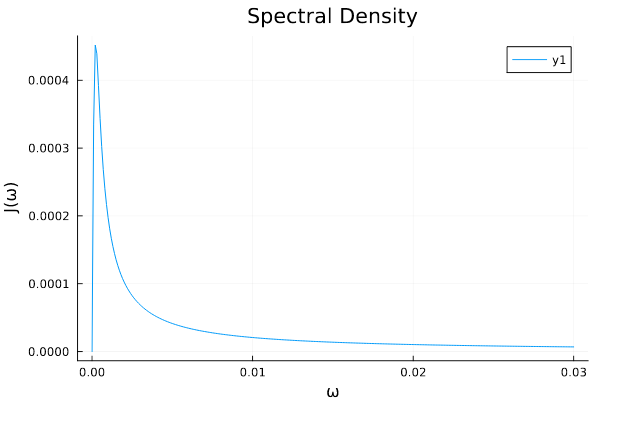
\includegraphics[scale=0.3]{Figures/jw_pentacene.png}
    \caption{Debye Spectral Density for Pentacene}
\end{figure}

Using calculations from the Quasi-Adiabatic Propagator Path Integral method, we can see the propagation of the density matrix. We can use this data to obtain the populations of the various sites (diagonal elements) and the coherences between the sites (off-diagonal elements).

\begin{figure}[h]
\centering
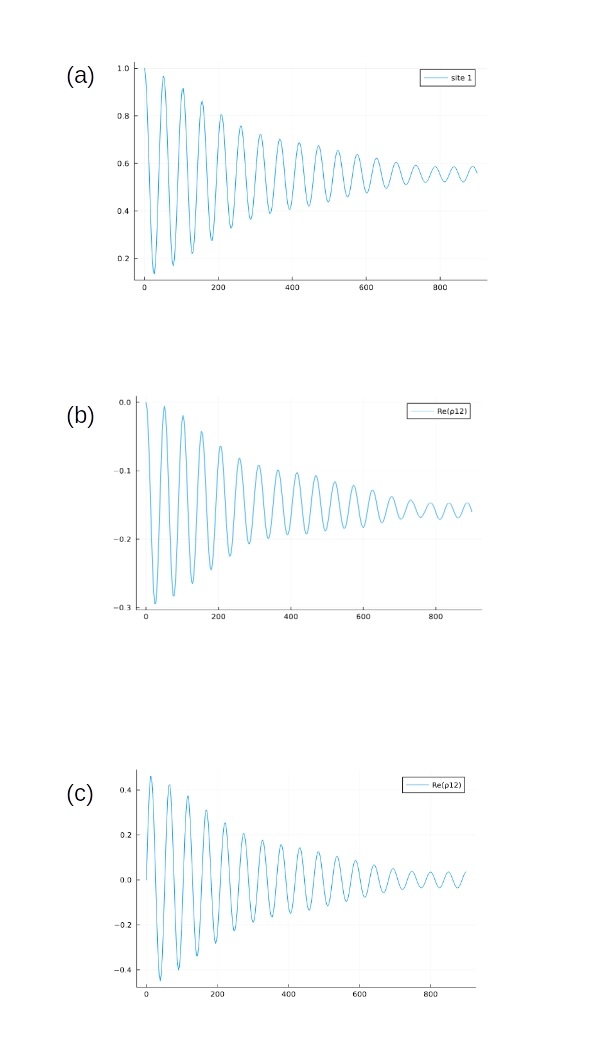
\includegraphics[scale=0.4]{Figures/pentacene_result}
\caption{Density Matrix Elements of Pentacene dimer. (a) $\rho_{11}$ population of site 1 (b) $Re(\rho_{12})$ Real part of coherence (c) $Im(\rho_{12})$ Imaginary part of coherence}
\end{figure}

%\begin{figure}
%\centering
%\includegraphics[scale=0.4]{Figures/pentacene_result2}
%\caption{Density Matrix Elements of Pentacene tetramer. (a) $\rho_{11}$ population of site 1 (b) $Re(\rho_{12})$ Real part of coherence (c) $Im(\rho_{12})$ Imaginary part of coherence}
%\end{figure}



\section{Rubrene}

Here, we attempt to model the dynamics of the Holstein-Peierls polaron in rubrene using the model developed by Ordejon, et al \cite{Ordejn2017}, where the Hamiltonian is given by :

\begin{equation}
    \mathcal{H} = \sum_{M,N} \epsilon_{MN} a_M^{\dag}a_N + \sum_{Q = (Z,P)} \omega_{Q} (b_Q^{\dag} b_{Q} + \frac{1}{2}) + \sum_{Q, M, N} \omega_{Q} g_{MN}^{Q}(b_{-Q} + b_{Q}^{\dag})a_M^{\dag}a_N 
\end{equation}

The effects of the bath are taken into consideration by the spectral density $J(\omega) = \sum_{i} g_i ^{2} \delta(\omega - \omega_i)$. We use a Gaussian line-shape broadening to model the spectral density $J(\omega)$.


\begin{figure}
    \center
    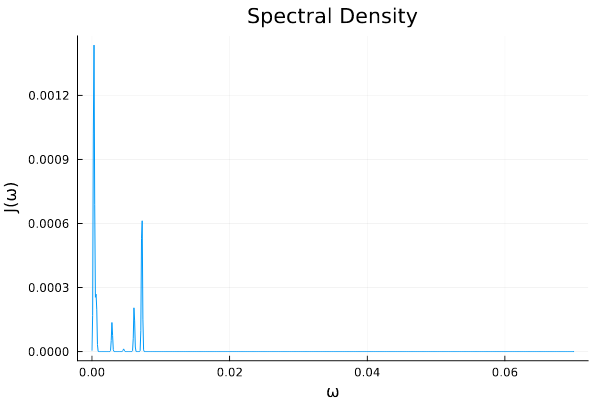
\includegraphics[scale=0.4]{Figures/jw_rubrene.png}
    \caption{Spectral Density (with Gaussian broadening) for Rubrene}
\end{figure}

We consider a simplified 1-dimensional chain of 10 rubrene sites with interactions between the nearest 2 neighbours.

By evaluating the QuAPI integral using tensor-train Monte carlo computations, we obtain the values of the RDM elements over time. We can use the diagonal elements to get the site populations.

\begin{figure}[h]
    \centering
    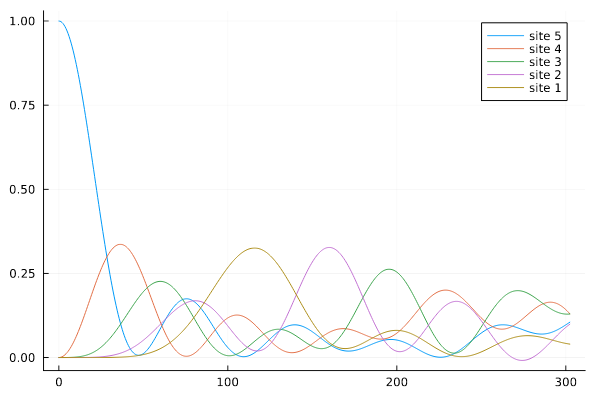
\includegraphics[scale=0.4]{Figures/rubrene_result.png}
    \caption{Populations of various sites in rubrene over time}
\end{figure}







%\input{Chapters/Chapter4}
%\input{Chapters/Chapter5}
%\input{Chapters/Chapter6}
%\input{Chapters/Chapter7}

%-------------------------------------------------------------------------------
%	THESIS CONTENT - APPENDICES
%-------------------------------------------------------------------------------

\addtocontents{toc}{\vspace{2em}} % Add a gap in the Contents, for aesthetics


\label{Bibliography}


\printbibliography

\end{document}
